\subsection{Chiral effects}

\begin{itemize}
	\item
The vacuum of quantum chromodynamics (QCD) is characterized by rich geometry structure which may corresponds to the fractal-like geometry \cite{IJMPE-22-1350041-2013}.There is a fundamental interrelation between geometry and essential properties of QCD Lagrangian.
Structures with non-trivial topology in QCD vacuum are believed to determine the behavior of the $\mathcal{P / CP}$ fundamental symmetries in the hot quark-gluon matter. Due to higher luminosity at the HL--LHC and / or high multiplicity per event at HE--LHC energy the multiparticle azimuthal correlations can be used for investigations of wide set of chiral effects in strong interaction \cite{PAN-80-1133-2017}, for instance, chiral magnetic effect -- CME, chiral magnetic waves -- CMW etc. This approach  allows the significant suppression of the backgrounds and improvement of reliability of physical conclusions. The study of charge-dependent azimuthal correlations for various types of light flavor particles can be possible with unprecedented precision due to high luminosity of the HL--LHC project. Consequently the quantitative comparison will be allowed for strengths of correlations in meson, baryon--meson and baryon systems. Such measurements will be essential in particular for search for chiral vortical effect -- CVE and its study with high precision. Furthermore the higher energies of the HE--LHC project can provide the opportunity for study of flavor dependence of the $\mathcal{P / CP}$ violation with help the azimuthal correlations for wider set of types of secondary particles including for heavy flavor ones. Thus experimental study of topology of QCD vacuum can be one of the focuses for studies of bulk properties within the HL--LHC, HE--LHC projects.
\end{itemize}



\begin{figure}[!htb]
\begin{center}
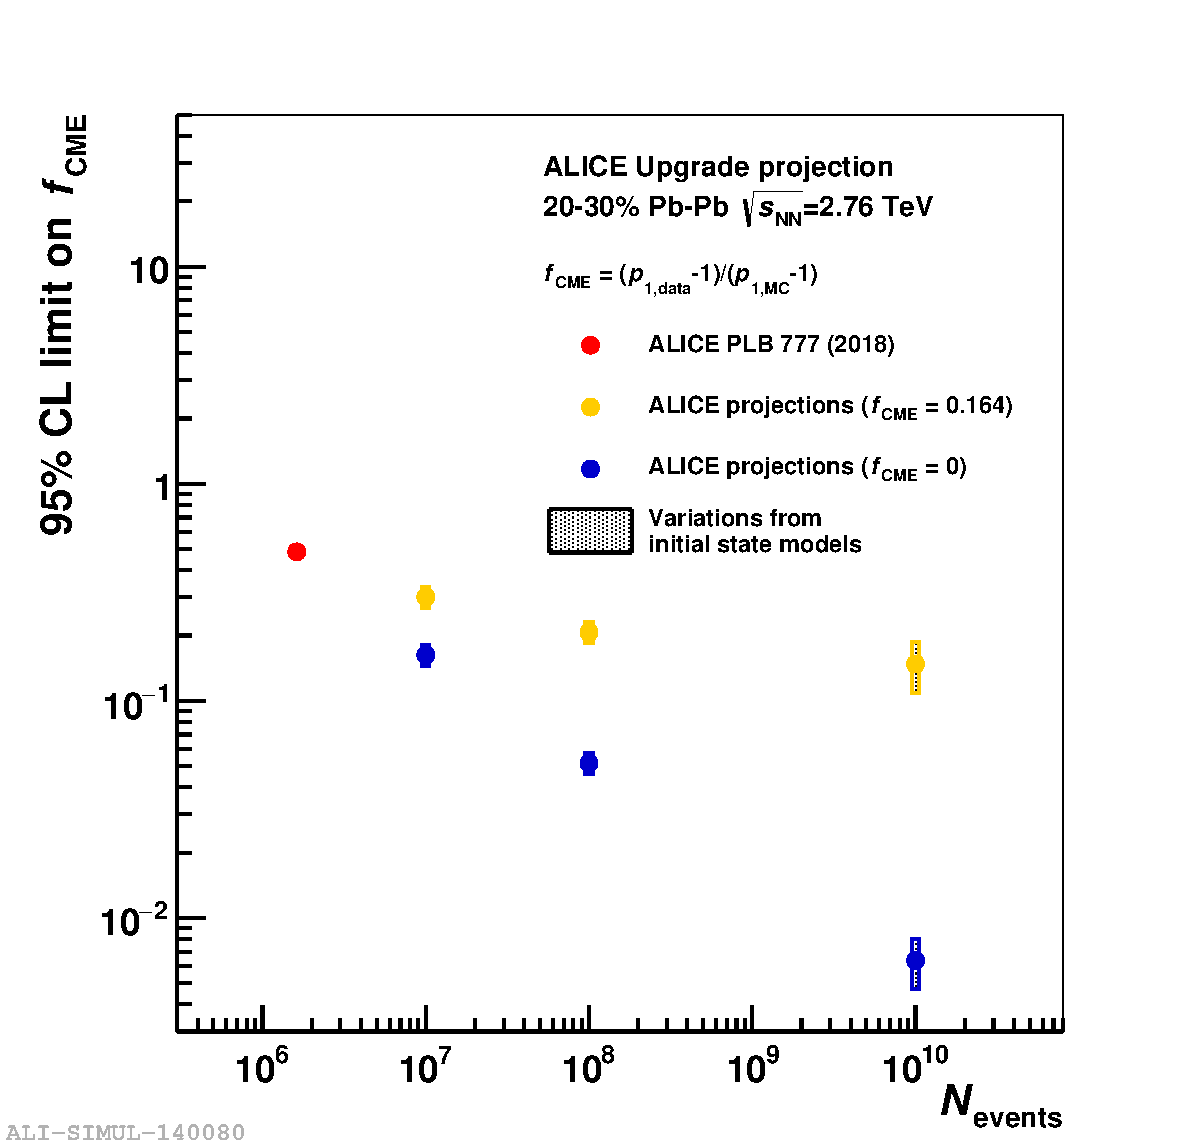
\includegraphics[width=0.8\textwidth]{\main/flow/figs/alice_projection_fcme}
\caption{
}
\label{fig:alice_fcme}
\end{center}
\end{figure}

